\RequirePackage[l2tabu,orthodox]{nag}

% TODO: decide if one-sided/two-sided
%\documentclass[headsepline,footsepline,footinclude=false,fontsize=11pt,paper=a4,listof=totoc,bibliography=totoc,BCOR=12mm,DIV=12]{scrbook} % two-sided
\documentclass[headsepline,footsepline,footinclude=false,oneside,fontsize=11pt,paper=a4,listof=totoc,bibliography=totoc]{scrbook} % one-sided

% TODO: change citation style in settings
\input{settings}

% TODO: change thesis information
\newcommand*{\getUniversity}{Technische Universität München}
\newcommand*{\getFaculty}{Department of Informatics}
\newcommand*{\getTitle}{Skeleton Prediction of 3D Biomedical Structures}
\newcommand*{\getTitleGer}{Skelettprognose von 3D Biomedizinisch Strukturen}
\newcommand*{\getAuthor}{Alok Verma}
\newcommand*{\getDoctype}{Master's Thesis in Biomedical Computing}
\newcommand*{\getSupervisor}{Prof. Dr. Laura Leal-Taixé}
\newcommand*{\getAdvisor}{Prof. Dr. Hanspeter Pfister and Dr. Donglai Wei}
\newcommand*{\getSubmissionDate}{April 15, 2020}
\newcommand*{\getSubmissionLocation}{Munich}

\makeatletter
\DeclareOldFontCommand{\rm}{\normalfont\rmfamily}{\mathrm}
\DeclareOldFontCommand{\sf}{\normalfont\sffamily}{\mathsf}
\DeclareOldFontCommand{\tt}{\normalfont\ttfamily}{\mathtt}
\DeclareOldFontCommand{\bf}{\normalfont\bfseries}{\mathbf}
\DeclareOldFontCommand{\it}{\normalfont\itshape}{\mathit}
\DeclareOldFontCommand{\sl}{\normalfont\slshape}{\@nomath\sl}
\DeclareOldFontCommand{\sc}{\normalfont\scshape}{\@nomath\sc}
\makeatother
\newcommand{\eg}{\textit{e}.\textit{g}.}
\newcommand{\etall}{\textit{et al.}}
\begin{document}

% Set page numbering to avoid "destination with the same identifier has been already used" warning for cover page.
% (see https://en.wikibooks.org/wiki/LaTeX/Hyperlinks#Problems_with_Links_and_Pages).
\pagenumbering{alph}
\input{pages/cover}

\frontmatter{}

\input{pages/title}
\input{pages/disclaimer}
\addcontentsline{toc}{chapter}{Acknowledgments}
\thispagestyle{empty}

\vspace*{20mm}

\begin{center}
{\usekomafont{section} Acknowledgments}
\end{center}

\vspace{10mm}

I would like to thank Prof. Hanspeter and Donglai at Harvard for hosting and guiding me, Prof. Laura at TU Munich for accepting my thesis proposal and being so supportive throughout it.

\cleardoublepage{}

\chapter{\abstractname}

To understand the internal workings of brain neuroscientists have been trying to reconstruct its 'neural circuitry', also termed as a 'connectome' which illustrates how neurons are connected with each other. 

A connectome can be constructed by segmenting neurons in a 3D electron microscopy(EM) image and then by finding their inter-connections. Past decade has seen increasing use of Deep Learning based methods to improve segmentation of such EM images and it has been quite indispensable in improving the state of the art in EM segmentation. 

But the neuron tracing problem is a hard problem to solve in itself. This can be attributed to its large volume size, multiple image artifacts, numerous closely intertwined segments of vivid shapes etc. \textcolor{red}{show images illustrating problems}. Hence, the results of most algorithms are either not satisfactory or they are too slow and entail complicated postprocessing steps, limiting their scope to only inside a computer science lab, and far away from being used as a general tool directly by neuroscientists for new images.

This work tries to develop a new idea of building connectomes, bypassing the segmentation step. It builds upon from existing methods and approaches in EM segmentation but also leverages the tools and tricks of Machine Learning methods from natural image domain. 

The first part discusses the relevant works from the Connectomics area, their advantages and pitfalls. Apart from that, it also delves into skeletonization methods used for natural images, which inspires the
proposed method.








\microtypesetup{protrusion=false}
\tableofcontents{}
\microtypesetup{protrusion=true}

\mainmatter{}

% !TeX root = ../main.tex
% Add the above to each chapter to make compiling the PDF easier in some editors.

\chapter{Introduction}\label{chapter:introduction}

\section{Connectomics}
To understand the internal workings of brain neuroscientists have been trying to reconstruct its 'neural circuitry' also termed as a connectome, which illustrates how neurons are connected with each other. The first ever brain to be studied at this intricate detail was that of C. Elegans in the 1980's ~\cite{whiteCElegans} with serial section electron microscopy(EM) images and the neurons were traced manually. 

Since then, EM methods have improved many folds, generating petabytes of data, even for a small Fruit Fly brain\textcolor{red}{cite Drosophilia paper}. So, the process of segmenting and tracing neurons have been delegated to Machine Learning(ML) algorithms, with humans pitching in only for error correction or initial training data generation. 

Neuron tracing problem is a hard nut to crack. This can be attributed to its large volume size, multiple image artifacts, numerous closely intertwined segments of vivid shapes etc. \textcolor{red}{show images illustrating problems}. Hence, the results of most algorithms are either not satisfactory or they are too slow and entail complicated postprocessing steps, limiting their scope to only inside a computer science lab far away from being used as a tool directly by neuroscientists.

This work tries to build upon from existing method and approaches which researchers have been working on from deca


\section{Connectomics Pipeline}

%\begin{figure}[htpb]
%  \centering
%  \newcommand{\mywidthSmall}{0.15\textwidth}
%  \newcommand{\mywidth}{0.20\textwidth}
%  \newcommand{\myheight}{0.20\textwidth}
%  \newcolumntype{X}{ >{\centering\arraybackslash} m{\mywidth} }
%  \setlength\tabcolsep{3mm} 
%  \def\arraystretch{0}%  1 is the default
%  \begin{tabular}{XXX}
%    \includegraphics[height=\myheight, width=\mywidthSmall,keepaspectratio]{data/images/brain.png}&
%    \includegraphics[height=\myheight, width=\mywidth,keepaspectratio]{data/images/slicing.jpg}&
%	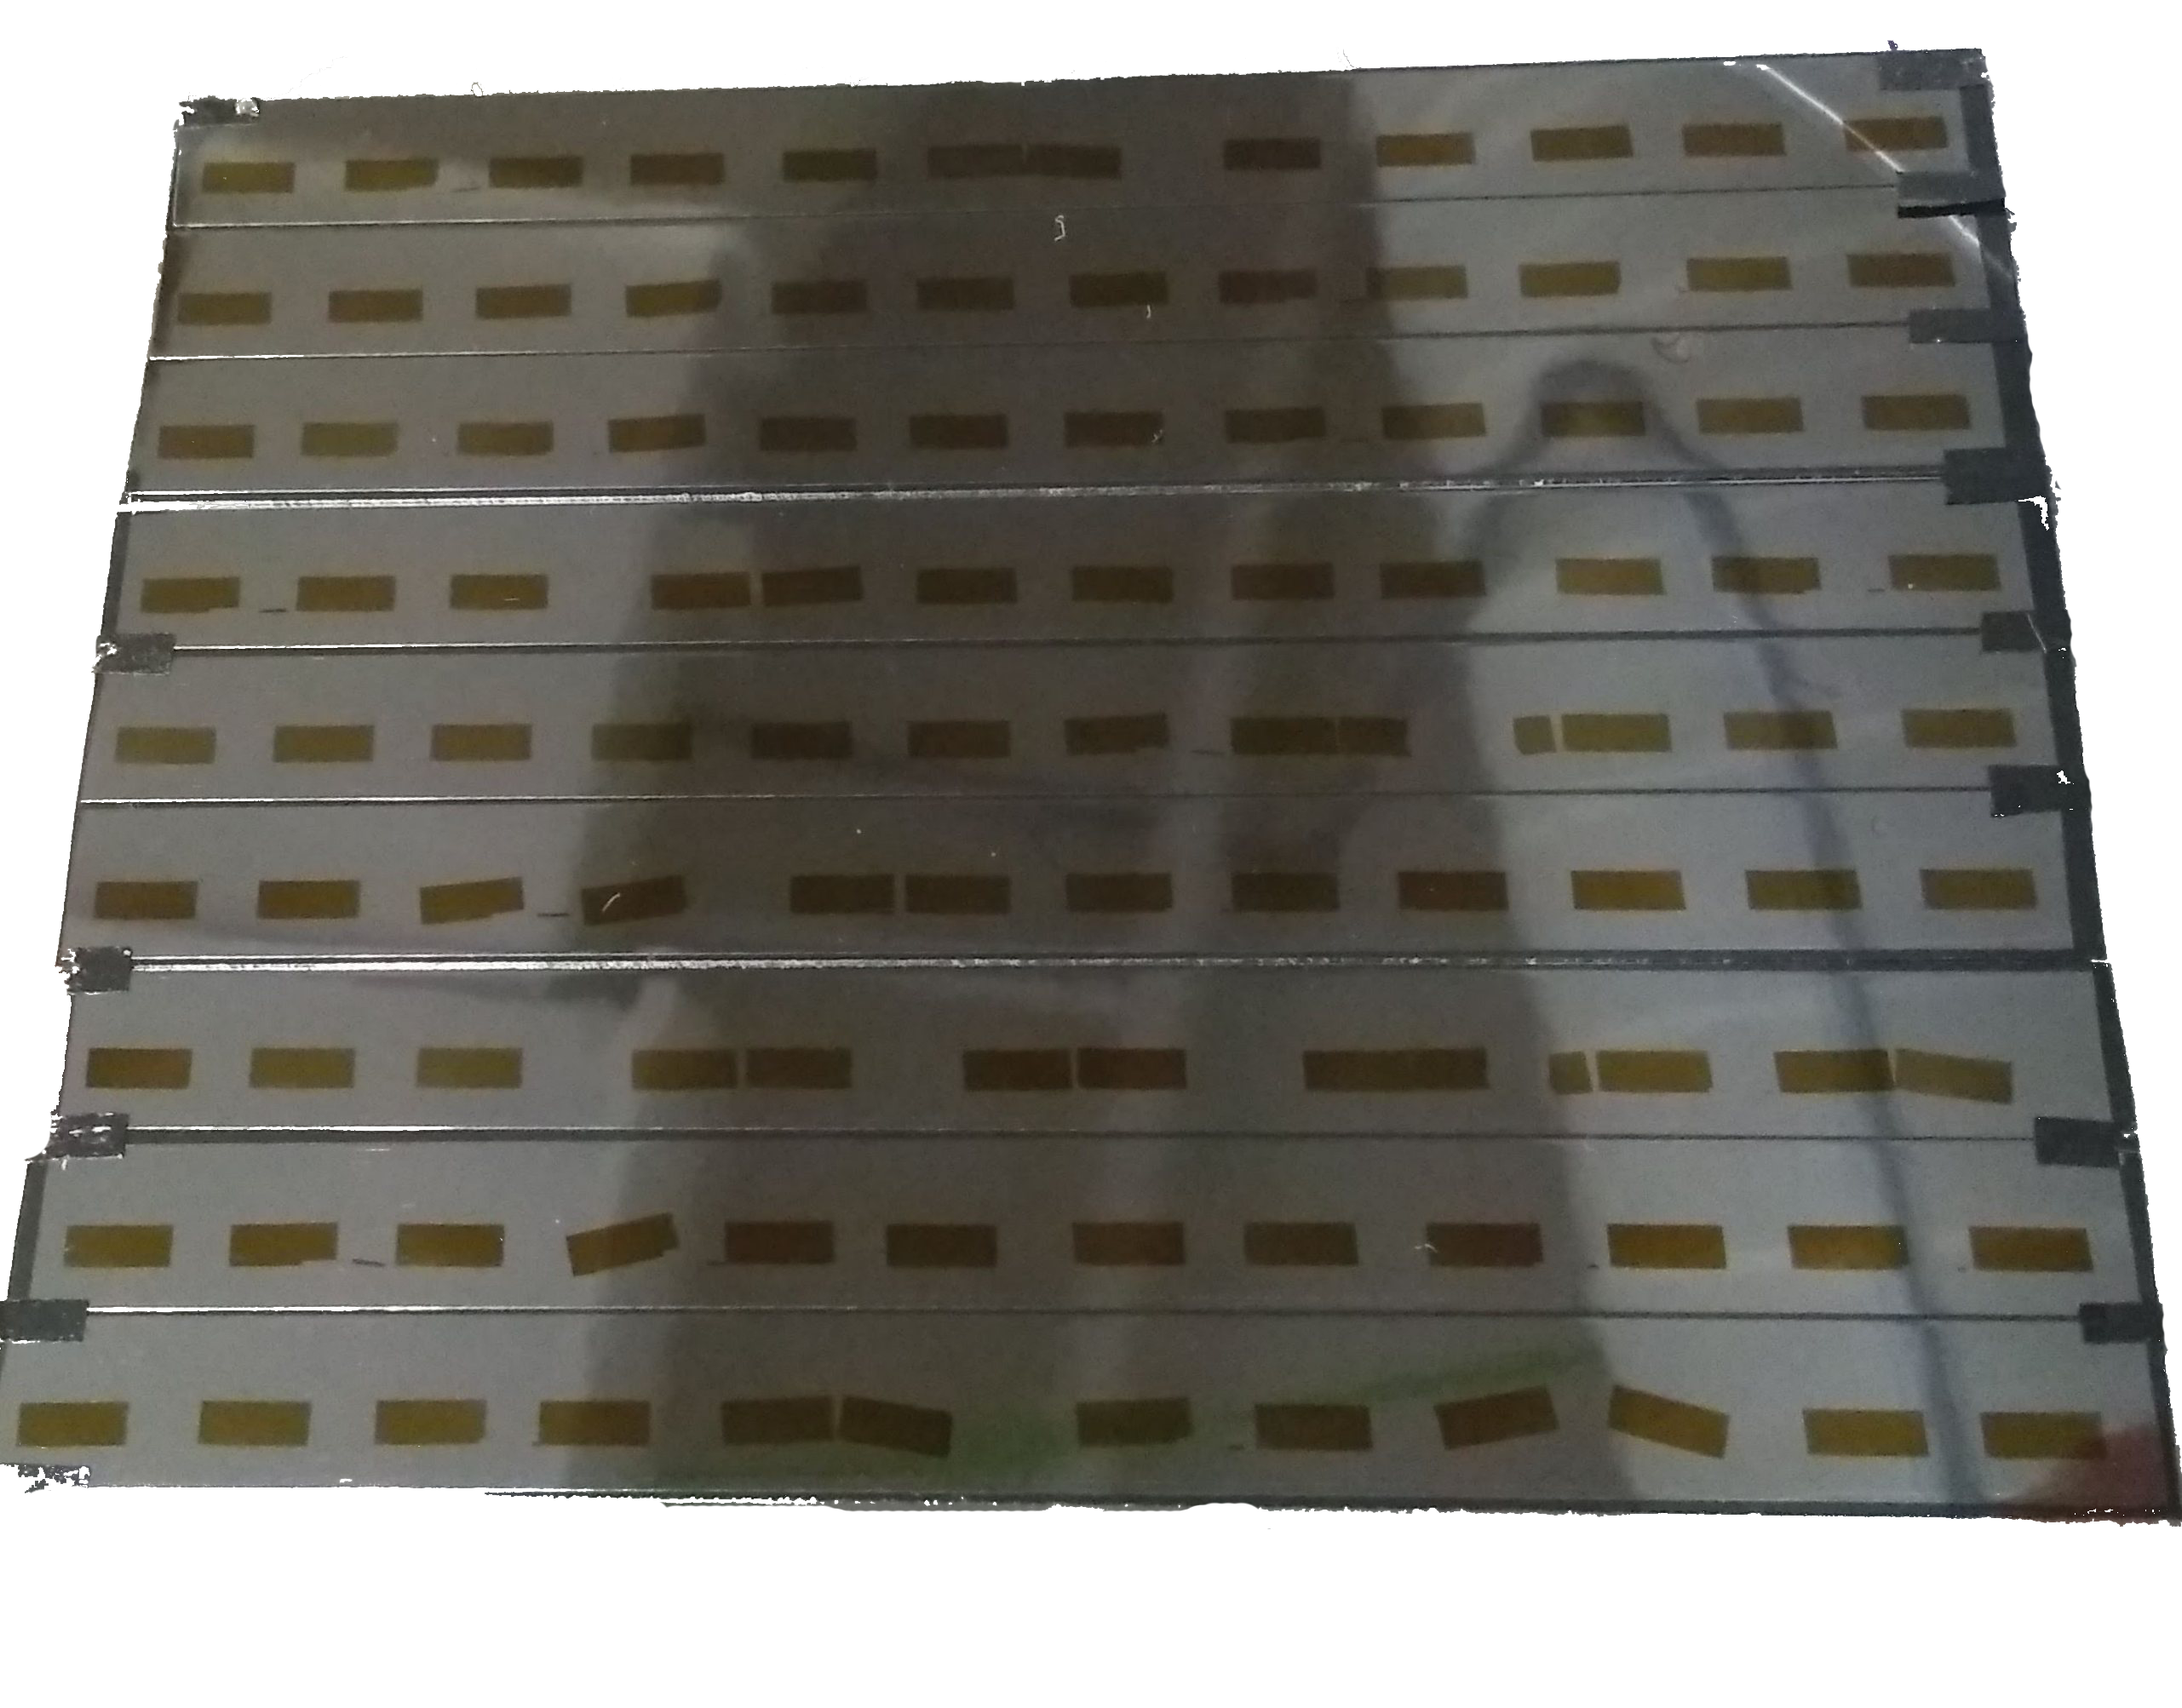
\includegraphics[height=\myheight, width=\mywidthSmall,keepaspectratio]{data/images/slices.png}\\
%	%\includegraphics[height=0.1\textheight,width=\mywidth,keepaspectratio]{data/images/emMicroscope.jpg}&
%	\includegraphics[height=\myheight,width=\mywidth]{data/images/imStack.png}&
%	\includegraphics[height=\myheight,width=\mywidth]{data/images/segStack.png}&
%	\includegraphics[height=\myheight,width=\mywidth]{data/images/seg3d.png}\\
%  \end{tabular}
%	\caption{Connectomics Pipeline.}
%	\label{fig:connectomicsPipeline}
%\end{figure}

\begin{figure}[htpb]
	\newcommand{\mywidth}{0.44\textwidth}
	\centering
	\begin{subfigure}[b]{\mywidth}
		\centering
		\includegraphics[width=\textwidth]{data/images/slicing/slicing_diagram.png}
		\caption{\label{fig:slicing_diagram}}
	\end{subfigure}
	\hspace{3mm}
	\begin{subfigure}[b]{\mywidth}
		\centering
		\includegraphics[width=\textwidth]{data/images/slicing/slicing.png}
		\caption{\label{fig:slicing}}
	\end{subfigure}
	\hspace{3mm}
	\begin{subfigure}[b]{\mywidth}
		\centering
		\includegraphics[width=\textwidth]{data/images/slicing/slicing_close.png}
		\caption{\label{fig:slicing_close}}
	\end{subfigure}
	\hspace{3mm}
	\begin{subfigure}[b]{\mywidth}
		\centering
		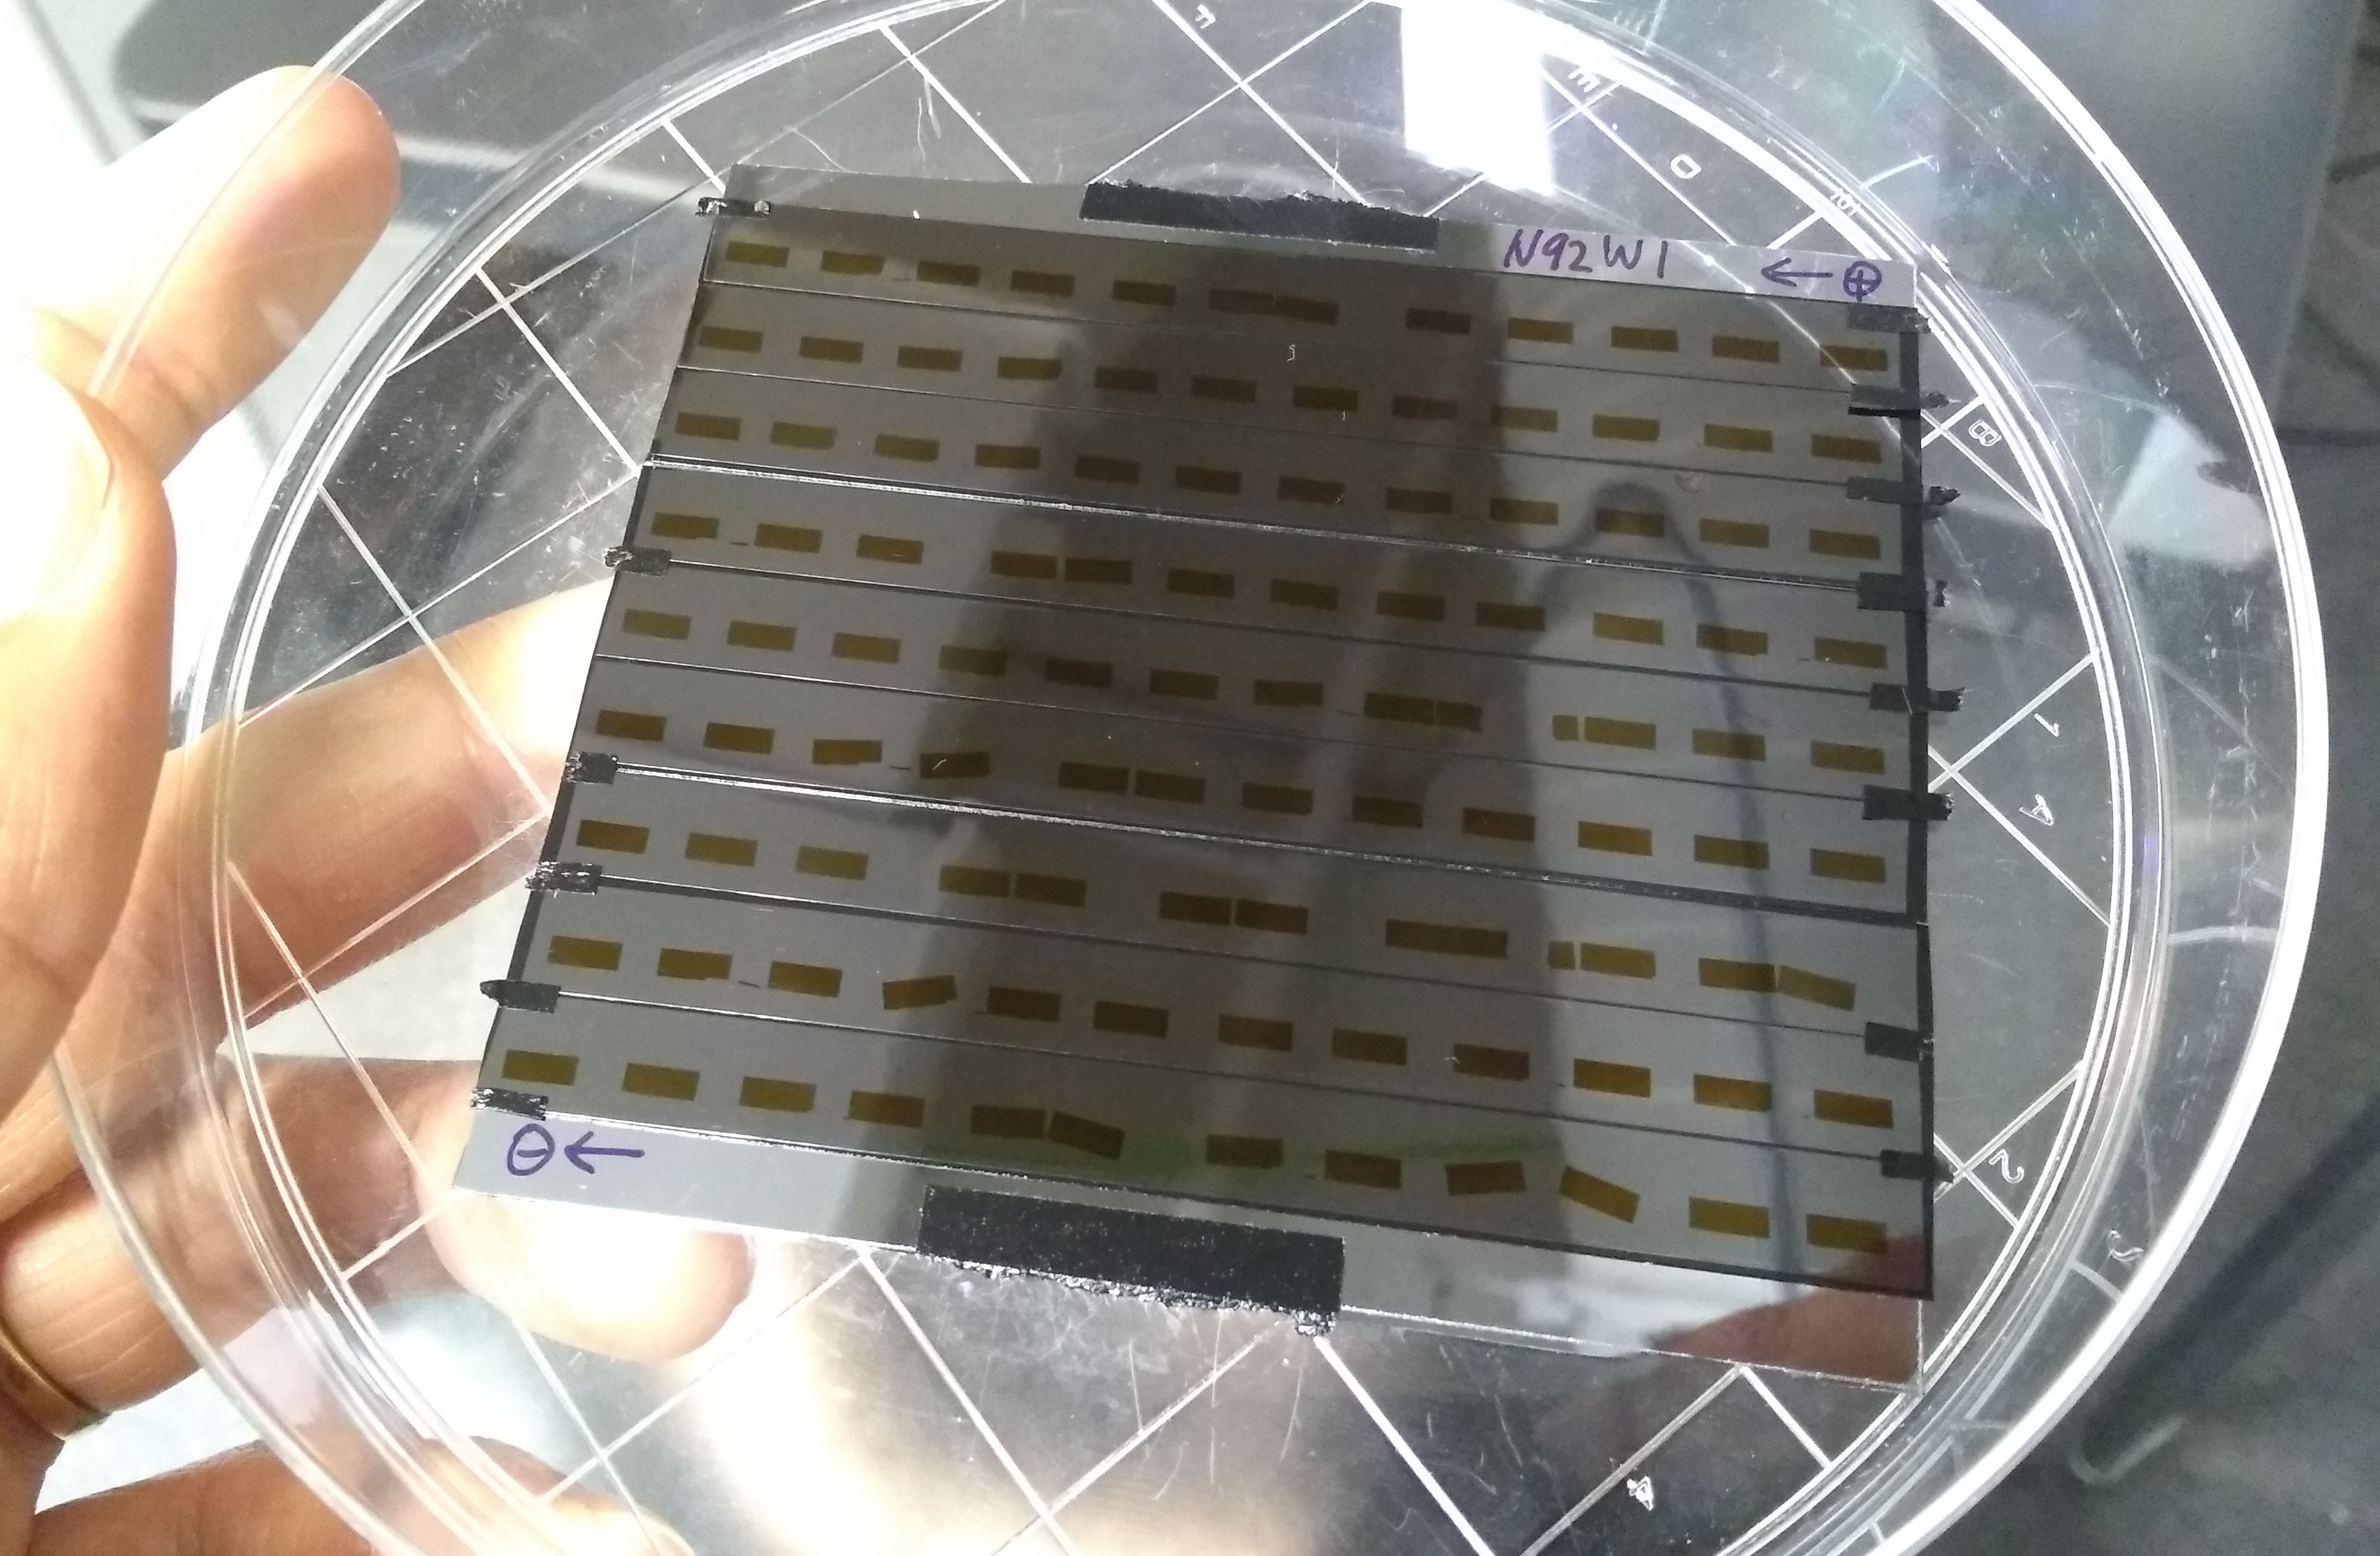
\includegraphics[width=\textwidth]{data/images/slicing/wafer.png}
		\caption{\label{fig:wafer}}
	\end{subfigure}
	\caption{Automated high-throughput serial sectioning setup. \subref{fig:slicing_diagram} explains a automated serial sectioning setup \cite{Baena2019}, \cite{Hayworth2006}. \subref{fig:slicing} shows a similar setup at Lichtman Lab, Harvard. \subref{fig:slicing_close} shows thin rectangular slices being collected on the conveyor tape. \subref{fig:wafer} shows a set of slices on wafer, later to be imaged using an electron microscope. All images are courtesy of Lichtman Lab \cite{LichtmanLab} and its members.}
	\label{fig:emSlicing}
\end{figure}

\begin{figure}[htpb]
	\newcommand{\mywidth}{0.44\textwidth}
	\newcommand{\mywidthlarge}{0.66\textwidth}
	\centering
	\begin{subfigure}[b]{\mywidth}
		\centering
		\includegraphics[width=\textwidth]{data/images/stack/im.png}
		\caption{\label{fig:im_stack}}
	\end{subfigure}
	\hspace{3mm}
	\begin{subfigure}[b]{\mywidth}
		\centering
		\includegraphics[width=\textwidth]{data/images/stack/seg.png}
		\caption{\label{fig:seg_stack}}
	\end{subfigure}
	\hspace{3mm}
	\begin{subfigure}[b]{\mywidthlarge}
		\centering
		\includegraphics[width=\textwidth]{data/images/stack/seg_3d.png}
		\caption{\label{fig:seg_3d}}
	\end{subfigure}
	\caption{3D EM image stack and segmentation. \subref{fig:im_stack} shows stacking of a few aligned 2D images along $Z$ axis. Alignment can be tough due to image artifacts and deformations during slicing. \subref{fig:seg_stack} shows the corresponding segmentation map created manually. Annotators glance across multiple slices to figure tougher segment boundaries. \subref{fig:seg_3d} shows the final manual segmentation output.}
	\label{fig:emSegmenting}
\end{figure}

The construction of the brain connectomes starts by slicing the brain tissue as thin as possible and imaging the 2D slices using an electron microscope, typically at resolution of $3 - 10$ nanometers. After imaging, the 2D images are stacked, aligned and processed to remove noise and other artifacts.\textcolor{red}{cite alignment papers, ask Adi}. Finally, this 3D image is segmented, often by doing multiple, laborious iterations of automatic segmentation and manual error correction to obtain a connectivity graph of the neuronal processes. Figure \ref{fig:connectomicsPipeline} shows a simplified succinct connectomics pipeline, starting from the brain tissue, alignment and segmentation. After segmentation multiple other analysis can be performed, which would entail more processing.


\section{Quirks of EM Data}
A Electron Microscopy(EM) image stack can contain numerous of segments which are arbitrarily and closely intertwined with each other. The membranes demarcating different cells can be thin and tough to distinguish even by trained humans. \autoref{fig:snemiDataset} shows a EM dataset \textcolor{red}{cite SNEMI} illustrating thin boundaries, closely packed nature of those neuronal segments and intertwined structure of the segments.

Apart from previously mentioned properties, EM datasets especially from serial section EM usually have some more quirks like:
\begin{itemize}
  \item The resolution of the 3D image may not be isotropic. For serial section EM, the in-plane resolution along $X$ and $Y$ axis is usually $2$ to $5$ times higher than the $Z$ resolution which is governed by the slice thickness 
  \item 2D image slices can have large artifacts due to physical folds or knife marks while imaging.
  \item There can be sharp discontinuities across slices due to misalignment, missing slices etc.
  \item The boundaries of segments can break at some points or get blurred and hard to distinguish.
  \item The size in pixels of one volume can be in the order of $10K*10K*5K$ voxels and a single segment can encompass from one diagonal end to the other.
\end{itemize}

Thus, EM datasets are much more complex to segment compared to other natural non medical imaging datasets, and thus specialized algorithms need to be developed to tackle them.


\begin{figure}[htpb]
  \centering
  \newcommand{\mywidth}{0.4\textwidth}
  \newcommand{\myheight}{0.3\textwidth}
  \newcommand{\mywidthLarge}{0.3\textwidth}
  \newcommand{\myheightLarge}{0.3\textwidth}
  \newcolumntype{X}{ >{\centering\arraybackslash} m{\mywidth} }
  \setlength\tabcolsep{3mm} % default value: 6pt
  \def\arraystretch{0}%  1 is the default
  \begin{tabular}{XX}
	\includegraphics[height=\myheight,width=\mywidth, keepaspectratio]{data/images/snemiGlimpse/snemiTrainSliceImages.png}\caption*{2D image slice.}&
	\includegraphics[height=\myheight,width=\mywidth,keepaspectratio]{data/images/snemiGlimpse/snemiTrainSliceLabels.png}\caption*{2D segmentation} \\
	\includegraphics[height=\myheight,width=\mywidth,keepaspectratio]{data/images/snemiGlimpse/snemi3DSeg.png}\caption*{3D segmentation.}&
	\includegraphics[height=\myheight,width=\mywidth,keepaspectratio]{data/images/snemiGlimpse/snemi3DSkelContext.png}\caption*{3D skeletons.}
  \end{tabular}
	\caption{The SNEMI Dataset. It was created as part of a Connectomics challenge to advance segmentation methods \textcolor{red}{Cite SNEMI}. The dimensions are relatively small - $100*1024*1024$ voxels with resolution of $30*6*6$ nm. }
	\label{fig:snemiDataset}
\end{figure}


\section{Segmentation Methods}

\subsection{Boundary based Methods}
To segment multiple 3D segments as shown in \autoref{fig:snemiDataset} one of the usual methods is to first perform semantic segmentation into two classes - foreground, which consists of all the internal pixels of segments, and background, which consists of the extracellular space. Given such a perfect semantic mask, it is trivial to obtain the instance segmentation of each cell using simple connected component analysis. One can then match segments from different slices using intersection of union scores. \textcolor{red}{cite boundary matching paper} \textcolor{blue}{ask donglai how boundary mask is segmented?}

Another commonly used approach for EM 3D segmentation is to represent boundaries as affinity graphs, first introduced by \cite{Turaga2010}. In its simplest form affinity graphs are similar to boundary masks - if a voxel and its immediate next neighbor lie in same segment then a high value, usually $1$, is stored at that voxel. In this scenario the affinity graph would be of $3$ channels, one each for the immediate next neighbour along $X$, $Y$ and $Z$. Affinity graphs can be created for distant neighbors also, leading to more channels, and encoding long distance connectivity, useful for thin elongated segments, used by \cite{Kisuk2017}. After obtaining such soft partition graph, the final segmentation can be done using standard graph partitioning methods or even connected components analysis, as shown in \cite{Turaga2010} or 3D affinity based watershed transform, used by \cite{Kisuk2017} and \cite{Aleks2015WatershedClustering}.

A common underlying idea in both methods is that they break down the segmentation problem into two steps. First is a local prediction step, where boundary is predicted based on local image textures and edges. Second is somewhat more global, which looks at connectivity of voxels and performs hierarchical clustering of oversegmented clusters based on shape and connectivity. The dismantling of the segmentation problem helps to tackle multi instance segmentation problem and makes it amenable for Deep Learning (DL) based methods.

A major issue with these pipeline processes is that a minute leak in the boundary segmentation can lead to false merge. To somewhat avoid such false merges, the hyper-parameters of watershed clustering are tuned so as to keep the results optimally over-segmented. This is done keeping in mind that its easier to correct false splits for humans rather than fixing false merges. Nevertheless, manually agglomerating over-segmentation is still laborious and not extendable to larger volumes.
Second issue, encountered in DL based boundary prediction methods with a $L1$ or $L2$ loss is that it cannot force the network to learn the shape of segments, a cue very frequently used by human annotators to distinguish ambiguous boundaries. This is due to the fact that we are only forcing the network to learn local boundary predictions, which a model can learn to predict based on textures only which is not enough.
Apart from this, models are trained to reduce the mean loss over the entire dataset, this means it may learn to generate boundaries for most parts of the segment correctly, but may miss some boundaries. Even those small errors can snowball into large false merges in post-processing steps as explained earlier. \textcolor{red}{Show images for segmentation error cases?}. Recently, structured loss for 3D EM segmentation was proposed to avoid this \cite{Funke2019}. It penalizes erroneous affinity predictions which can lead to false merges or splits. 

\subsection{Error detection and Error Correction}
It is unrealistic to obtain perfect boundary predictions directly from a single Deep Net. For perfect boundary prediction an enormous corpus of training data and a versatile loss function is needed, which forces the network to learn to look for higher order cues like continuity across slices, shape of 3D segments etc, and not just texture. So, recent works have explored the idea of error detection and correction of pre-segmented volumes \cite{Seung2017}, \cite{Brain2019}. \cite{Seung2017} trains a model to first identify split and merge errors and then trains another model for creating a correct segmentation at those locations. While, \cite{Brain2019} solves false splits by computing skeletons and searching for matching skeletons near its ends. It computes a weighted graph with nodes comprising of segments and edges weighted by the probability of segments being merged together. The merges are finally computed by a graph partitioning algorithm.

\subsection{Flood Filling Network}
All the previous discussed methods\textcolor{red}{cite segmentation papers}  were tuned and tested on relatively small scale data, but advancements in EM helped create larger and larger datasets reaching hundreds of Gigabytes, and the previous state-of-the-art couldn't catch up to produce acceptable results. But a recent method called Flood Filling Network (FFN) \cite{Januszewski2018FFN} from Google was able to produce acceptable results for the first time on volumes of approx size $10K*10K*6K$ voxels.
Their method segments one object at a time, growing its mask sequentially, until it traces the entire object. Initially a small seed is marked inside a segment, and a mask is predicted using a Deep Net for that single segment in a small field of view around that seed, further seed points are found inside the predicted mask by jumping a fixed step size in all possible directions.
But similar to previous approaches neither can this method predict a mask completely accurately in one-shot. So, multiple iterations are run at different scales and seeding order to create a over-segmentation and then an extensive agglomeration step is performed using the same model.
It is interesting to note that while this method is the state-of-the-art in connectomics, but apparently no other lab than Google has been able to use it for any large dataset. One reason being, with just $1000$ P100 GPUs it needs $16$ hours to run inference on the large volume\cite{Januszewski2017FFN}. So, currently its hard to put forth FFN as a general tool for Neuroscientists and a urgent need remains to create a segmentation tool which is feasible and easy to use.

\section{Skeletons in Connectomics}
While EM segmentation is a major step in the connectomics challenge but it is not the final goal. Neuroscientists are interested to find out interconnections between neurons, identify common neurons shapes \cite{Zhao2014}, find geodesic distance between synapse connections and soma etc. Such analysis naturally calls in for skeletonization of neurons, and a straight forward way is to skeletonize the predicted segmentations, for which many off the shelf algorithms already exist \cite{TEASAR}, \cite{Palagyi2014}. Recently, skeletonization methods specially curated for EM data have also been proposed \cite{Brian2019Skel}. 
Apart from serving as a connectome analysis tool, skeletons are instrumental in improving the segmentations itself. Since, they capture a global topology of segments - branch points and end points - they can be a indicator of false split and false merges in segmentation\textcolor{red}{Show picture of FM and FS in skeletons?}. A recent method \cite{Brain2019} utilized skeleton end points to identify false splits and merged them using skeleton curvature information.
Creating ground truth skeleton data is also easier than segmentations. Dedicated tools \cite{KNOSSOS} exist for human annotators for neuron center line labelling. One paper \cite{Berning2015} quotes manual skeletonization to be $25$ to $100$ times faster than segmentation labelling. It also proposes a semi-automatic segmentation method based on hand traced neurons. 
Also, the state-of-the-art FFN method, \cite{Januszewski2017FFN}, \cite{Januszewski2018FFN} utilizes skeletons for validation and error metric (estimated run length) calculation. The metric they choose is tailored to report high error if the reconstructed segmentations are falsely merged or split, but it does not penalize small segmentation perturbations on the boundary, so the focus is more on improving the topology - or the centerline skeletons - rather than boundaries.
In another kind of neural images obtained from Fluorescence confocal microscopy, Neuron tracing \cite{Kayasandik2018} methods are being developed, which essentially is also skeletonization.
So, skeletons are a useful representation for neurons and would be an important tool for EM connectomics in near future.

\subsection{Skeletonization in 2D Natural images}
Since many natural image processing tools have been applied to EM images, it is pertinent to review existing 2D natural image to skeleton methods which can guide development of 3D EM skeletonization method. 

It would come as no surprise that all recent state of the art methods \cite{Shen2016}, \cite{Shen2017}, \cite{Ke2017}, \cite{Wang2019}, \cite{Xu2019}
are based on deep learning. Except \cite{Wang2019}, all cited methods formulate skeltonization as a pixelwise binary classification problem. \cite{Shen2016}, \cite{Shen2017}, \cite{Ke2017} utilize multiple side outputs from different depths of the network to capture skeletons at different scales. They use cross entropy loss for training, which is easy to backpropagate, but does not focus on any skeleton shape regularization, leading to blurry and disconnected predictions.
\cite{Wang2019} on the other hand proposes to learn a vector field called flux, which points to the nearest skeleton pixel. A decoding step is required to extract skeletons from the field. 
\cite{Xu2019} argues against such field prediction and proposes geometry aware loss function which penalizes blurry and disconnected outputs.
% !TeX root = ../main.tex
% Add the above to each chapter to make compiling the PDF easier in some editors.

\chapter{Method}\label{chapter:method}

A novel method for instance skeletonization of neuronal structures in EM images is proposed. The method is motivated by existing learning based skeletonization method for natural images \cite{Wang2019}, but differs in two distinct ways. First, it separates skeletons for each individual segment - we describe it as instance skeletonization. Second, its is applied on 3D EM images instead of 2D images, which, to the best of our knowledge, has not been explored yet. 
 
\section{Encoding Skeletons in a Vector Field}
Previous skeletonization methods \cite{Shen2016}, \cite{Shen2017}, \cite{Ke2017}, \cite{Wang2019}, \cite{Xu2019} do not separate skeletons of multiple objects. Their prediction is a binary mask marking skeleton points of all salient objects as 'True'. But, in EM images, it is important to separate skeletons of one object instance from another. 
But, it is not straight forward to construct a single Deep Net which can directly demarcate skeletons of object instance. Hence, a encoding must be devised which allows formulating a feasible loss metric and also simple intuitive postprocessing step for decoding skeleton instances. 

\cite{Wang2019} proposes 'Deep Flux' which encodes skeletons of objects in 2D images using a $\mathbb{R}^2$ vector field. It defines a 2D context region around skeleton, and all $\mathbb{R}^2$ vectors in that context region point to the nearest skeleton pixel. This provides a encoding to represent skeletons, and the objective of a Deep Net model would be to predict this field.

The proposed method is also inspired from this encoding, albeit for 3D skeletons and some other tweaks.

Given, ground truth skeletons, a context region is defined for each skeleton, which are the set of points inside a $3D$ ball of $r$ radius.
Let $\Omega \subset \mathbb{Z^3}$  be the 3D image domain consisting of points $\mathbf{p}: (x, y, z)$ and ${\Omega}_s \subset \Omega$ be the set of skeletons points manually labeled. The context set, ${\Omega}_c$ of the skeletons can be defined as

\DeclarePairedDelimiter\norm\lVert\rVert

\begin{equation}
{\Omega}_c := \{ \mathbf{p} \in \Omega \vert \min_{\mathbf{q} \in \Omega_s} \norm{\mathbf{p} - \mathbf{q}}_2 < r \} 
\end{equation}

Further a distance transform $D$ is defined from the skeleton points inside the domain $\Omega$ as

\begin{equation}
\mathbf{D}(\mathbf{p}) := \begin{cases}
		\min_{\mathbf{q} \in \Omega_s} \norm{\mathbf{p}-\mathbf{q}}_2 & \text{if } \mathbf{p} \in \Omega_c \\
		0  & \text{otherwise}
		\end{cases} 
\end{equation}

Finally a $\mathbb{R}^3$ vector field, $\overline{D}$ is obtained by taking discrete gradient of $D$ as follows

\begin{equation}
 \overline{\mathbf{D}}(\mathbf{p}) := \begin{cases}
 \nabla \mathbf{D} & \text{if } \mathbf{p} \in \text{int } \Omega_c \\
 0  & \text{otherwise}
 \end{cases} 
\end{equation}
 
In essence $\overline{\mathbf{D}}$ is a vector field with non-zero direction vectors defined in the vicinity of skeletons, such that the vectors are pointing away from the skeletons, as shown in \autoref{fig:context_field_directions}.

\begin{figure}[htpb]
	\newcommand{\mywidth}{0.45\textwidth}
	\centering
	\begin{subfigure}[b]{\mywidth}
		\centering
		\includegraphics[width=\textwidth]{data/images/contextField/context2D.png}
		\caption{\label{fig:context}}
	\end{subfigure}
	\hspace{3mm}
	\begin{subfigure}[b]{\mywidth}
		\centering
		\includegraphics[width=\textwidth]{data/images/contextField/directions_skel_context.png}
		\caption{\label{fig:directions_skel_ctx}}
	\end{subfigure}
		\caption{\subref{fig:context} shows the context for skeletons in a 2D slice. \subref{fig:directions_skel_ctx} shows the field vectors inside the context. They all point away from the skeletons and also follow the shape of the skeleton smoothly}
		\label{fig:context_field_directions}
\end{figure}
	
But, such defined direction field is non-smooth if the skeletons are defined on a discrete grid, shown in \autoref{fig:splineInterpolation}. Learning such a non-smooth field is not encouraged as Deep Nets are usually fail to generate such sharp fields. Hence, to create smoother field, skeleton points are interpolated using splines. Hence, $\Omega_s \subset \mathbb{R}^3$.

\begin{figure}[htpb]
	\newcommand{\mywidth}{0.22\textwidth}
	\centering
	\hspace{3mm}
	\begin{subfigure}[b]{\mywidth}
		\centering
		\includegraphics[width=\textwidth]{data/images/interpolation/slice_edited.png}
		\caption{\label{fig:3dseg_slice}}
	\end{subfigure}
	\hspace{3mm}
	\begin{subfigure}[b]{\mywidth}
		\centering
		\includegraphics[width=\textwidth]{data/images/interpolation/linear_skel.png}
		\caption{\label{fig:skel_linear}}
	\end{subfigure}
	\hspace{3mm}
	\begin{subfigure}[b]{\mywidth}
		\centering
		\includegraphics[width=\textwidth]{data/images/interpolation/spline_skel.png}
		\caption{\label{fig:skel_spline}}
	\end{subfigure}\\
	\hspace{3mm}
	\begin{subfigure}[b]{\mywidth}
		\centering
		\includegraphics[width=\textwidth]{data/images/interpolation/seg_slice.png}
		\caption{\label{fig:im_seg}}
	\end{subfigure}
	\hspace{3mm}
	\begin{subfigure}[b]{\mywidth}
		\centering
		\includegraphics[width=\textwidth]{data/images/interpolation/dtx_linear.png}
		\caption{\label{fig:dtx_linear}}
	\end{subfigure}
	\hspace{3mm}
	\begin{subfigure}[b]{\mywidth}
		\centering
		\includegraphics[width=\textwidth]{data/images/interpolation/dtx_spline.png}
		\caption{\label{fig:dtx_spline}}
	\end{subfigure}\\
	\hspace{\mywidth}
	\hspace{3mm}
	\begin{subfigure}[b]{\mywidth}
		\centering
		\includegraphics[width=\textwidth]{data/images/interpolation/gradz_linear.png}
		\caption{\label{fig:grad_linear}}
	\end{subfigure}
	\hspace{3mm}
	\begin{subfigure}[b]{\mywidth}
		\centering
		\includegraphics[width=\textwidth]{data/images/interpolation/gradz_spline.png}
		\caption{\label{fig:grad_spline}}
	\end{subfigure}
	\caption{ \subref{fig:skel_linear} and \subref{fig:skel_spline} are resulting skeletons for linearly and spline interpolation methods respectively. \subref{fig:im_seg} is a segment slice in $X-Y$ plane sliced as shown in \subref{fig:3dseg_slice}. \subref{fig:dtx_linear} and \subref{fig:dtx_spline} are the normalized isotropic 3D distance transform from the skeleton for linearly and spline interpolated versions respectively. \subref{fig:grad_linear} and \subref{fig:grad_spline} shows the $z$ component of the gradient of \subref{fig:dtx_linear} and \subref{fig:dtx_spline} respectively. Sharp fields exist in \subref{fig:grad_linear} due to artifacts in the distance transform in \subref{fig:dtx_linear}.}
	\label{fig:splineInterpolation}
\end{figure}


The advantages for encoding skeletons in such a field are:
\begin{itemize}
	\item Deep Net model has to learn to look for both global and local properties while predicting the field. This helps to avoid local false merges due to small membrane breaks, as seen in boundary based methods.
	\item Voxel wise loss function for the deep net can be easily constructed. The loss metric is agnostic of skeleton instances.
	\item Predicted field can be useful to solve false merges and splits in later post processing steps.
\end{itemize}

\section{Network Architecture}
Input to the network is a grayscale image and output is 3 channel vector field.
The backbone of the network is based on Unet \cite{ronneberger2015}. The encoder and decoder of the Unet has four stages, and a center bottleneck layer, with $8, 16, 24, 32, 40$ filters respectively. Each stage of Unet consists of a 3D convolution layer and a residual block. Each residual block made up of two 3D convolution layers with kernel size 3, a short skip connection and ELU nonlinearity. Since EM images have anisotropic resolution, the first and the last stages of the Unet has only 2D convolutions. This is done keeping in mind that first stage can extract information from the high resolution 2D slices and later stages can combine them to extract higher level of information and be resistant to inter-slice artifacts. For downsampling and upsampling in encoder and decoder, 3D Maxpool and linear upsampling is used with a factor of 2, with an exception in the first the last stage where 2D Maxpooling and linear upsampling is used. The network has a theoretical field of view of \textcolor{red}{378*378*32, calculate this again}.  

\section{Training Objective}
Though a L2 or L1 loss between target field $\mathbf{T}$ and predicted field $\mathbf{P}$ can be used, but a more stringent loss would be to enforce correct prediction of the directions of the vectors. This forces a sharper prediction and ensures that the network directly learns directions and hence the shape of the neurons. But since, outside the context region of skeletons the vector field has zero magnitude and thus directions are meaningless. So, a weighted combination (\autoref{loss}) of mean square error(\autoref{mse}) and cosine loss (\autoref{cosineLoss}) is used.

\begin{equation}\label{cosineLoss}
\mathcal{L}_{cos}(\mathbf{P}, \mathbf{T}) := \sum_{\mathbf{q} \in \Omega} \mathbf{W}(\mathbf{q})\left( 1 - \frac{\mathbf{P}(\mathbf{q}).\mathbf{T}(\mathbf{q})}{\max(\norm{\mathbf{P}(\mathbf{q})}_2.\norm{\mathbf{T}(\mathbf{q})}_2,\,\epsilon)} \right)
\end{equation}

\begin{equation} \label{mse}
\mathcal{L}_{mse}(\mathbf{P}, \mathbf{T}) := \sum_{\mathbf{q} \in \Omega} \mathbf{W}(\mathbf{q}) \norm{\mathbf{P}(\mathbf{q}) - \mathbf{T}(\mathbf{q})}_2^2
\end{equation}

\begin{equation} \label{loss}
\mathcal{L} := \alpha\mathcal{L}_{cos} + (1-\alpha)\mathcal{L}_{mse}
\end{equation}

\begin{figure}[htpb]
	\newcommand{\mywidth}{0.3\textwidth}
	\centering
	\begin{subfigure}[b]{\mywidth}
		\centering
		\includegraphics[width=\textwidth]{data/images/fieldLearning/fi_image.png}
		\caption{\label{fig:fi_im}}
	\end{subfigure}
	\hspace{3mm}
	\begin{subfigure}[b]{\mywidth}
		\centering
		\includegraphics[width=\textwidth]{data/images/fieldLearning/fi_im_field.png}
		\caption{\label{fig:fi_im_f}}
	\end{subfigure}\\
	
	\begin{subfigure}[b]{\mywidth}
		\centering
		\includegraphics[width=\textwidth]{data/images/fieldLearning/fi_field.png}
		\caption{\label{fig:fi_f}}
	\end{subfigure}
	\hspace{3mm}
	\begin{subfigure}[b]{\mywidth}
		\centering
		\includegraphics[width=\textwidth]{data/images/fieldLearning/fi_result.png}
		\caption{\label{fig:fi_r}}
	\end{subfigure}
		
	\caption{\subref{fig:fi_im} and \subref{fig:fi_f} shows an 2D slice of input data and the ground truth field. They are overlayed in \subref{fig:fi_im_f}. \subref{fig:fi_r} shows the predicted field.}
	\label{fig:learnedField}
\end{figure}

\section{Decoding Skeletons from Vector Field}
To obtain the instance skeletons back from such an encoding, simple postprocessing steps can be used. First observation about the predicted field is: in the vicinity of skeleton voxels they point away from each other, while at non skeleton voxels they point almost in the same direction. This property can be used to identify skeleton voxels. Divergence at skeleton points would be high, where as for all other location it would be low. And thus thresholding the divergence would allow to create a skeleton mask. Finally, for separating instance skeletons, connected components analysis can be performed.

\section{Splitting and Matching}
After connected component analysis, instance skeletons of most cells can be obtained. But, some skeletons of small and closely located segments are falsely merged, also some skeletons are broken due to irregular shapes and artifacts. To improve such skeletons, another post processing step is devised. 
All false merges occur as junction points of skeletons. So, Junction points are located and the skeletons are split at those locations by a cutting plane along the two eigen vectors with least eigen value.
This results in over-split skeletons, but with almost no false merges.
Finally to merge split skeletons, a classifier is trained to predict if a pair of skeleton requires to be merged. The input to the classifier is a small cropped 3D volume of EM image around the center of the two end points of the skeleton, also combined with it are the cropped skeletons mask in separate channels and the predicted field.

\begin{figure}[htpb]
	\centering
	\begin{subfigure}[b]{0.3\textwidth}
		\centering
		\includegraphics[width=\textwidth]{data/images/matchingData/positive_2.png}
		\caption{\label{fig:positiveMatch}}
	\end{subfigure}
	\hspace{3mm}
	\begin{subfigure}[b]{0.3\textwidth}
		\centering
		\includegraphics[width=\textwidth]{data/images/matchingData/negative_2.png}
		\caption{\label{fig:negativeMatch}}
	\end{subfigure}
	\caption{Positive \subref{fig:positiveMatch} and negative \subref{fig:negativeMatch} training samples for training a classifier to merge skeletons. Each red line in \subref{fig:negativeMatch} pairs two skeletons which are not part of the same segment. Green line in \subref{fig:positiveMatch} represent the skeleton parts from same segment which needs to be matched}
	\label{fig:skelMatchTrainData}
\end{figure}


\begin{figure}[htpb]
	\centering
	\begin{subfigure}[b]{0.24\textwidth}
		\centering
		\includegraphics[width=\textwidth]{data/images/splitNMatch/skel.png}
		\caption{\label{fig:splitNMatchA}}
	\end{subfigure}
	\hfill
	\begin{subfigure}[b]{0.24\textwidth}
		\centering
		\includegraphics[width=\textwidth]{data/images/splitNMatch/skelNSeg.png}
		\caption{\label{fig:splitNMatchB}}
	\end{subfigure}
	\hfill
	\begin{subfigure}[b]{0.24\textwidth}
		\centering
		\includegraphics[width=\textwidth]{data/images/splitNMatch/split.png}
		\caption{\label{fig:splitNMatchC}}
	\end{subfigure}
	\hfill
	\begin{subfigure}[b]{0.24\textwidth}
		\centering
		\includegraphics[width=\textwidth]{data/images/splitNMatch/matched.png}
		\caption{\label{fig:splitNMatchD}}
	\end{subfigure}
	\caption{Splitting and matching of skeletons. \subref{fig:splitNMatchA} and \subref{fig:splitNMatchB} shows the falsely merged skeletons. \subref{fig:splitNMatchC} shows skeletons after splitting. Notice that the colors of the skeletons have changed. \subref{fig:splitNMatchD} shows the classifier linking the correct skeletons parts together with yellow lines.}
	\label{skelSplitNMatch}
\end{figure}

% !TeX root = ../main.tex
% Add the above to each chapter to make compiling the PDF easier in some editors.

\chapter{Experiments}\label{chapter:experiments}

\section{Datasets}
We train and test proposed skeletonization method on three datasets.

\begin{itemize}
	\item \textbf{SNEMI3D} (\cite{SNEMI3D})- Originally a segmentation challenge organized to advance and compare automatic segmentation methods, has been used a benchmark for most automatic segmentation methods. As part of the challenge, a EM image of an adult mouse brain of size $100*1024*1024$ with a resolution of $6x6x30$ nanometer was manually annotated and released. The proposed method here requires skeletons for training, so thinning based skeletonization is applied on the ground truth segmentation to obtain skeletons. For test and validation a in-house manually labeled chunk from the same dataset \cite{Kasthuri2015}, of which SNEMI3D's dataset is part-of, is used.
	\item P7 - An in-house dataset of parallel fiber \textcolor{red}{Ask donglai about details}
\end{itemize}

\subsection{Evaluation Metric}
Previous 2D skeletonization methods \cite{Wang2019}, \cite{Xu2019} were agnostic of skeleton instances, so, the error metrics - Precision and Recall - were based on direct pixelwise calculation of true positive (TP), false positive (FP) and false negative (FN). 
In current proposed method skeletons for each segment are identified separately. This demands, first matching each proposed skeleton to a ground truth skeleton, similar to error metric proposed in \cite(Liang2019), which predicts road boundaries. Predicted skeletons are matched to one and only one ground truth skeleton instance based on its maximum overlap. Some predicted skeletons may not be matched to any ground truth, and vice versa. Precision and recall is then calculated, similar to \cite{Liang2019}, all predicted skeleton voxels within a threshold distance to ground truth skeleton is classified as TP, and rest as FP. FN are the voxels not in range of skeleton voxels. F1 score, harmonic mean of Precision and Recall is also reported.

To assess if predicted skeletons are over-split, a connectivity score is also calculated similar to \cite{Liang2019}.
% !TeX root = ../main.tex
% Add the above to each chapter to make compiling the PDF easier in some editors.

\chapter{Future Work}\label{chapter:further_work}
Our proposed method shows promising results for skeleton prediction in complicated 3D datasets but it still has unresolved false splits because the Tracking Network fails to correctly track in longer gaps. Also our splitting method creates more than necessary splits which could be avoided. So further work would be to:
\begin{itemize}
	\item Improve splitting process by selectively splitting at false splits. Currently all junction points are split but it is not necessary as some of them are branch points in the same object. A classifier can be designed to discriminate between false merges and branch points.
	
	\item Improve the training ground truth for Tracking Network. If there is a large mismatch between ground truth skeletons and predicted over-split skeletons the Tracking network may not learn meaningful filters. To alleviate this, synthetic Tracking Network ground truth can be constructed.
	
\end{itemize}

Also, one could find better error metrics for evaluating instance skeletonization performance since binary pixel level F1 score does not care about instances and even instance F1 scores are biased towards split skeletons. One potential candidate would be estimated run length metric from Januszewski \etall~\cite{Januszewski2017FFN, Januszewski2018FFN}.
Last, as an application for skeletons, skeleton-assisted segmentation methods can be devised which could alleviate false merges and splits in segmentation methods and also use cheaper skeleton labels for training.

% !TeX root = ../main.tex
% Add the above to each chapter to make compiling the PDF easier in some editors.

\chapter{Conclusion}\label{chapter:conclusion}

We developed an instance skeletonization method for 3D biomedical images and showed its efficacy on different modalities and complicated shapes.
We demonstrated our novel usage of topology of skeletons to resolve false merges which resulted in great improvement. While our method beats other state-of-the-art skeletonization approaches it still results in over-split skeletons. This means the splitting and tracking steps needs to be optimized further to achieve perfect results.

\appendix
% !TeX root = ../main.tex
% Add the above to each chapter to make compiling the PDF easier in some editors.

\chapter{Appendix}\label{chapter:appendix}

\section{Network Architectures}

\subsection{Flux Network}
Input to the network is a grayscale image and output is 3 channel vector field.
The backbone of the network is based on Unet \cite{ronneberger2015}. The encoder and decoder of the Unet has four stages, and a center bottleneck layer, with $8, 16, 24, 32, 40$ filters respectively. The network has a theoretical field of view of $32\times378\times378$. Further details can be seen in \autoref{fig:network_blocks} and \autoref{fig:flux_net}.

\begin{figure}[ht]
	\centering
	\includegraphics[width=\textwidth]{figures/network/legend.png}
	\caption{Network blocks used in Flux Network and Tracking Network.}
	\label{fig:network_blocks}
\end{figure}

\begin{figure}[ht]
	\centering
	\includegraphics[width=\textwidth]{figures/network/flux_net.png}
	\caption{Flux Network. Input is a grayscale image of size $1\times64\times192\times192$. Output is the flux field of size $3\times64\times192\times192$.}
	\label{fig:flux_net}
\end{figure}


\subsection{Tracking Network}

Tracking Network is based on 3D convolution layers, a convolutional LSTM block and fully connected layers at the end. The details are show in \autoref{fig:direction_net}.

\begin{figure}[ht]
	\captionsetup[subfigure]{aboveskip=1pt,belowskip=1pt}
	\centering
	\includegraphics[width=\textwidth]{figures/network/direction_net.png}
	\caption{Tracking Network. Input is a $14\times16\times64\times64$ volume, comprising of input image, flux, start skeleton mask, other skeletons mask, and global features from Flux Network of channel sizes $1, 3, 1, 1, 8$ respectively. Outputs are 1) growing direction vector of size 3 and a scalar for the \it{\{continue-stop\}} probability.}
	\label{fig:direction_net}
	\vspace{-0.1in}
\end{figure}


\microtypesetup{protrusion=false}
\listoffigures{}
\listoftables{}
\microtypesetup{protrusion=true}
\printbibliography{}

\end{document}
